We can now examine more closely the naming "monoclonal antibody": indeed, we
have to explain the difference between monoclonal and polyclonal antibodies,
and see why monoclonal antibodies are preferred to polyclonal antibodies
for therapeutic uses.

\begin{figure}[H]       
    \centering
    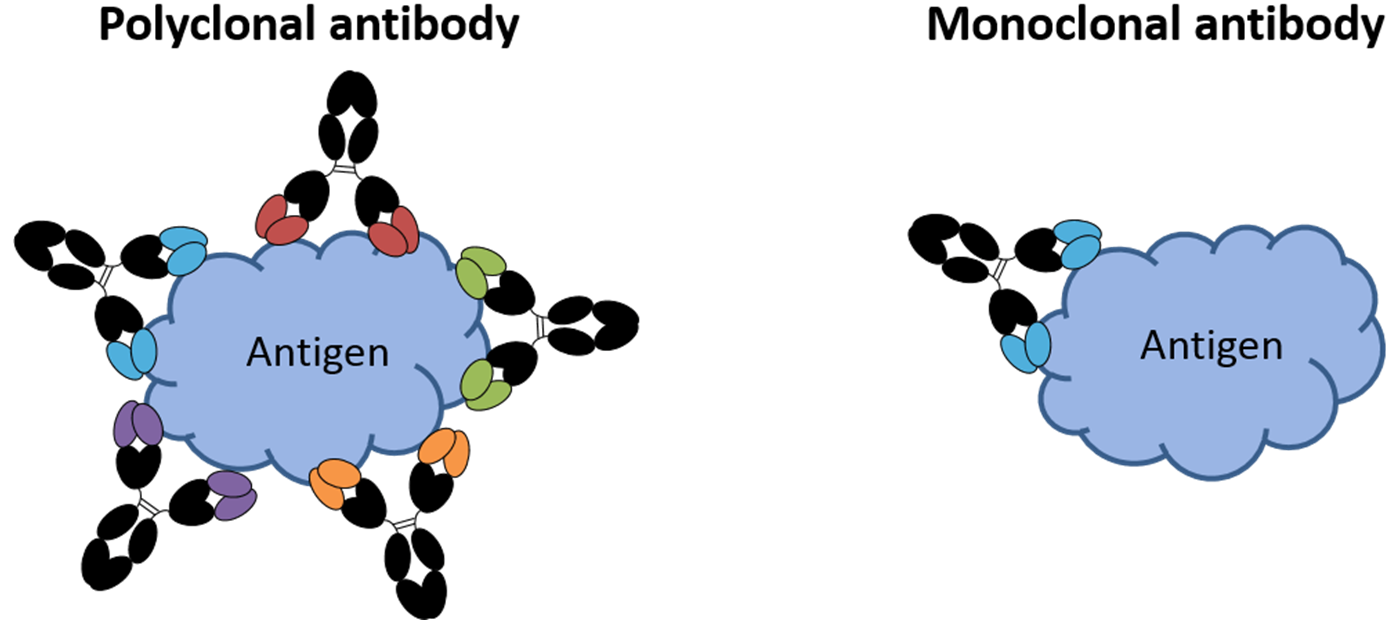
\includegraphics[width=0.6\textwidth]{../Images/Monoclonal_and_Polyclonal_Antibodies.png}   
    \caption{Schematic representation of monoclonal and polyclonal antibodies}
    \label{fig:Monoclonal_and_Polyclonal_Antibodies}
\end{figure}

First of all, let us define the two concepts :

\begin{itemize}
    \item \emph{Monoclonal antibodies} (mAbs) are antibodies produced from a single B-cell
    clone ; they are thus able to bind with a unique epitope of a specific antigen.
    \item \emph{Polyclonal antibodies} (pAbs) are antibodies produced from different B-cell
    lineages ; they form a collection of antibodies able to bind to a specific antigen
    by each identifying a different epitope.
\end{itemize}

Each of them have different advantages and disadvantages. Monoclonal antibodies
are homogeneous and consistent, allowing for a high concentration and purity,
as well as a reproducible production process \cite{lipman_monoclonal_2005}.
However, it is more complicated and thus more expensive to reach the production 
stage for mAbs, as we will see in part \ref{sec:monoclonal_antibody_production}.

On the other hand, polyclonal antibodies are simpler and cheaper to produce
on the short term \cite{nelson_monoclonal_2000}. PAbs are also less prone to
a reduction in efficiency if the epitope of the antigen has changed slightly
(for example by mutation of the targeted virus),
as they cover broadly the antigen with its multiple epitopes. However, since
pAbs are produced from animal of selected species, there is a batch-to-batch
variation meaning less long-term homogeneity \cite{nelson_monoclonal_2000}.
Moreover, it is observed that the resulting product is less concentrated and
pure than with mAbs \cite{lipman_monoclonal_2005}.

Finally, pAbs are well-suited for research purposes, allowing for quicker
development cycles. Monoclonal antibodies on the other hands are particularly
adapted for drug production as they offer great specificity to a selected antigen,
which is sought for when designing a drug, as it limits the probability of
having unpredicted side effects \cite{breedveld_therapeutic_2000}.
